\chapter{FPGA}
A powerfull Virtex-7 \gls{FPGA} Evaluation board VC707
was used to for the real time signal processing.
During this thesis the data from the \gls{ADC} is acquired and stored at in real
time and than passed to Matlab running on a personal computer to both test
the analog part of the system while keeping the fast implementation speed
and flexibility of Matlab to test the rest of the digital signal processing steps
of the receiver. Nevertheless the architecture was choosen such that it is easy
to step by step replace parts of the signal processing from Matlab to the
\gls{FPGA}.

\section{Architecutre Overview}
The three main tasks of the digital design are to acquire and store the data
produced by the \gls{ADC} in real time and to download this data to a
personal computer in a reasonable time for further processing. \\

As shown in \figref{fig:fpga_architecture_overview} the most important
modules of the design are the \verb|Adc12d1800| which interfaces the
\gls{ADC}, \verb|Ram| which uses a DDR3-\gls{RAM} to store the data
and \verb|Microblaze|, a soft-core processor, which controls the
\gls{USB} 2 data download. \verb|Data2Ram| is interface logic used
to connect the \gls{RAM} and \gls{ADC} and \verb|AxiSlave| implements
an interface between the Axi-Bus used by the Microblaze processor
and the custom \verb|Ram| module. \\

In the following sections each of this modules is shortly described followed
by some insights how clocking and reset is implemented.

\begin{figure}[ht]
  \centering
  %\includegraphics[width=\textwidth]{figures/}
  \caption{Overview of the architecture}
  \label{fig:fpga_architecture_overview}
\end{figure}

\begin{itemize}
\item Some words about where more receiver functions can be added
\item Req/Ack-protocoll, everything stallable
\end{itemize}

\section{Req/Ack Protocol}
\label{sec:fpga_reqack}
Between all modules a simple comminucation protocoll is used that allows
one way communication whenever the sender and the receiver are both
ready. As a consequence all module have to be stallable. By only using
one such protocoll arbitrary modules can often be connected
without any additional glue logic. \\

The protocol requires the sender to provide a request output which
is asserted if it has data to send. The receiver only than can apply
an assert output if its acknowledge output if it is ready to receive
the data in at the next positive clock edge. Data is transferred whenever
there is a positive clock edge and req and ack are both asserted (high). \\

Because the acknowledge output of a receiver by definition always depends on the
request input of a receiver, this leads to long chains of routing and
\gls{LUT} resources if not implemented well. Therefor a simple so called
req/ack breaker is used which adds one register into the data path. This results
in one cycle delay but makes the ack signal depending on a local register
only and not on the req signal. \\

This has also the advantage that long routing distances can be seperated by inserting
registers into the data and control path.

\todo{add reference to req/ack paper}

\section{Data Acquisition: Adc12d1800}
\label{sec:fpga_adc}

The \gls{ADC} Reference Board is connected to the Virtex-7 evaluation board using 
one of the two \gls{FMC} plugs. A listing of all connections can be found in
\secref{sec:app_adc_fpga_con}. \\

Data acquistions is done by the module \verb|Adc12d1800| which interfaces
the \verb|Adc12d1800rf| by Texas Instruments. In our case the ADC is configured
to sample two channels, an in-phase and a quadrature phase channel, at up to 1.8 GHz
or to sample one channel at 3.6 Ghz. The nominal resolution is 12 bits.
This results in a total bandwidth of $5.4 \text{Gb}/\text{s}$.
Since 1.8 GHz and especially 3.6 GHz is far beyond what the IO-Pads of all
\glspl{FPGA} \todo{reference needed} and most \glspl{ASIC} can handle,
the ADC can output on 4 parallel streams of 12 bit each. \\

Since this 4 streams might be routed with different wire lengths on a \gls{PCB}
each stream has it's clock aligned to the data.
In order to half the maximum frequency of the clock line to the same as the one
of the data lines, the data change on positive and negativ clock edges
(\gls{DDR}). \\

At full speed, this results in a switching frequency of 450 MHz for all data
and clock lines. To support this high speed while reducing power consumption,
and the influence of noise compared to classical \gls{CMOS} signaling,
\gls{LVDS} is used. \\

Since the maximum clock frequencies of the Virtex \glspl{FPGA} for logic
including \gls{LUT} slices and routings with fanouts above 4
are limited to around 200 to 300 MHz, the input stream needs to be further
parallelized. This desin uses a frequency of 250 MHz to output
the data of the \gls{ADC} for further processing. At this frequency
the only 4 ns are available between clock edges which is exeeded easily
as soon as a signal is routed far across the \gls{FPGA} die,
has a fanout of more than about 4, crossing clock domains leads
to clock skew or by more than about 3 logic slices between registers.
This makes the \gls{FPGA} design challanging since often multiple
complete synthesis, map, place \& route and timing analysis runs are
needed to find a design that meets timing. \\

As shown in \figref{fig:fpga_adc} the implemented design uses
a total of 5 stages to paralellize and concentrate the data to only
one single data rate stream following the req/ack protocol described in
\secref{sec:fpga_reqack}.

\subsection{Stage 0: Differential to Single-ended Conversion}
Each of the 12 bits and the clock of the 4 streams arrive at at the input bank
of the \gls{FPGA} at two neighbouring pads forming a \gls{LVDS} pair.
First this differential signal is converted to a single ended signal using
{\em Differential Signaling Input Buffer} (IBUFDS) primitives located next
to the pads. \\

This results in $4 \times 12$ bits single ended double data rates
signals plus 4 single ended clocks at up to 450 MHz.

\subsection{Stage 1: Double Data Rate to Single Data Rate Conversion}
\label{sec:fpga_adc_s1}
Next the first parallelization step is performed by outputing two new
bits on every positive clock edge instead of one on positive and negativ
clock edges. The Virtex-7 \gls{FPGA} have a dedicated hardware primitive
called {\em Input Dual Data-Rate Register} (IDDR) for this.
This primitives are placed next to the differential input buffers
and are automatically mapped correctly by the Xilinix tools. \\

This results in $4 \times 24$ bits of single ended single data rate
signals plus 4 single ended clocks at up to 450 MHz.

\subsection{Stage 2: Input FIFO}
Since 450 MHz is still beyond what can be routed through the general
routing resources and captured by registers, Xilinx added a special
{\em Input First-In, First-Out} primitive (IN\_FIFO)
directly into the IO-bank which can parallelize the data by a factor of two.
This primitive has a total of ten 4 bit wide input busses.
The primitive can be configured to concatenate two such input words
to one 8 bit wide output word and therefore provides a total of
ten 8 bit wide output words. \\

Four such IN\_FIFO are available for each
input/output bank consisting of a total of 50 pads aligned in a single row.
In our design each of the four 24-bit input streams is located at one
input/output bank and is routed to the inputs of one IN\_FIFO primitive.
Since the timing only holds if the instance in the middle of the bank
is used and the mapping tools map the IN\_FIFO instance to other
locations depending on the routings of the outputs, all those
IN\_FIFO primitives where manually constrained to the correct location. \\

Also these IN\_FIFO support an independed input and output clock.
As input clock the clock signals provides by the \gls{ADC} are each fed
into a so called {\em Advanced Mixed Mode Clock Manager} (MMCME2\_ADV).
This allows to arbitrarily shift the phases of the clocks to ensure
correct data capturing. The same clock was also used for the
IDDR-registers described in \secref{sec:fpga_adc_s1}. \\

For each input bank one such clock manager exists. To ensure that
always the one next to the input clock pads and the IN\_FIFO is
used, the four MMCME2\_ADV instances are also manually constrained to
one specific location. \\

This results in $4 \times 48$ bits of single ended single data rate signals.

\begin{figure}
  \centering
  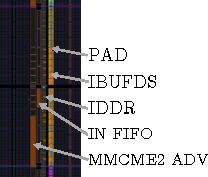
\includegraphics{figures/adc_input_bank}
  \caption{View of the pysical location of the primitives forming the
    \gls{ADC} interface on the \gls{FPGA}}
  \label{fig:fpga_architecture_overview}
\end{figure}

\subsection{Stage 3: Centralization and Reordering}
All previous stages were seperated for each of the four input streams
from the \gls{ADC} which are located at four different input banks.
Since the Input banks are distributed over the whole die, the data
has to be routed to one place first. This is done by allocating
three req/ack breakers (see \figref{fig:fpga_reaack_breaker})
for each of the four channels in a row allowing the tools a high flexibility
in allocating routing resources and putting registers in between.
All this req/ack breakers stall (ack not asserted) whenever the IN\_FIFO
is empty. \\

The four last req/ack breakers of the four channels are then connected
to one single req/ack breaker wich form the final output of the
\gls{ADC}-module. The data is order in such a way, that the final 192 bit
wide output vector is formatted as follows:
\[Q_7\;I_7\;Q_6\;I_6\;Q_5\;I_5\;Q_4\;I_4\;Q_3\;I_3\;Q_2\;I_2\;Q_1\;I_1\;Q_0\;I_0\]
Where $Q_t$ and $I_t$ are the quadrature channel repectively in-phase channel
12 bit words at time $t$.
The index $t$ is the time step where a higher number means later in time.
All the words are formatted with \gls{MSB} first.

\subsection{Testpattern generator}
For debugging purposes the \gls{ADC} interface has a built in test pattern
generator which outputs 16 words of 12 bit numbers in parallel such that
when lining up these 192 bit vectors this results in a continous count.

\section{Storage}
\label{sec:fpga_storage}
Whenever the arm signal (see \figref{fig:fpga_architecture_overview}) is asserted
by the Microblaze processor in charge of the download operation
(see \secref{sec:fpga_download}) and either a positive edge is detected
on the trigger input or the trigger button is pressed,
the \gls{RAM} of the \gls{FPGA} board is completely overwritten with new
\gls{ADC} samples. \\

The used \gls{RAM} module MT8JTF1286Hz offers is a standard \gls{DDR3} \gls{RAM}
and offers a total of 1 GiB of space devided into 8 banks of 128 MiB each.
This allows for parallel data transfers of 64 bits at speed of up to 800 MHz
resulting in a maximal bandwidth of $12.8 \text{GB}/\text{s}$. \\

Very similar to the \gls{ADC} data acquisition module (\secref{sec:fpga_adc})
this high clock rates can only be used very close to the input/output banks
and not for further routing and processing in the \gls{FPGA}.
For that purpose Xilinx provides a \gls{IP} core that on one end is connected
to the pads of the \gls{RAM} module and on the other side offers a user
friendly user interface on a in our case four times slower clock frequency.
It does so by taking care of address generation and refreshing the volatile
memory and uses parallelizaion to reduce the clock frequency of the user
interface. \\
\todo{add more information about what the difficulties of interfacing
ddr3 ram are}

Because place \& route turned out to be difficult at the maximal speed
of 800 MHz I used only 500 MHz as \gls{RAM} clock rate. This results
in a 512 bit wide user interface of the \gls{MIG} core running at 125 MHz
and a maximal bandwidth of $8 \text{GB}/\text{s}$. This is still slightly
higher than bandwidth of the \gls{ADC} and therefore allows realtime
storage of all data. Since there is 1 GiB \gls{RAM}
a total of $\approx 3.6 \codt 10^8$ complex samples can be saved. This
takes $\approx 190 \text{ms}$ at full \gls{ADC} speed. \\

Experiments showed that when consecutively writing to all addresses the
refresh needed refresh does not lead to any stalls and the full bandwidth
is available. Whenever, during the write requests, one sole read request
is perfomed, the user interface of the \gls{MIG} core stalls for about 11
cycles. This is not an issue though because in our case we first write
to all addresses, then stop writing and read out a part of the memory
at much lower speeds (see \secref{sec:fpga_download}). \\

Since the \gls{ADC} module outputs the data at 250 MHz in a 192 bit
wide vector and the \gls{RAM} module can write 512 bit wide vectors
at only 125 MHz a so called bus converter is used which concatenats
the 192 bits until at leas 512 bits are available. Behind this converter
a \gls{FIFO} memory is added to cross the clock boundry and to be able
to hold some samples when the \gls{MIG} user interface stalls. \\

During implementation care has to be exercised to the mask bits,
which are designed to prevent parts of the 64 bit written in parallel to be
overwritten and therefor allow for partial writtes without first performing
a read operation. Accidentally having these pins stuck at 1 due to
not connecting them prevents initialization and further reads from
working. \\

\section{Download}
\label{sec:fpga_download}
For further analysis and processing of the data captured by the \gls{ADC}
it should be sent to a personal computer.
Different options for downloading the 1 GiB of data from the \gls{FPGA}
to a computer were considered: \\

The simplest implementation would be to use
the CP2103GM USB-to-UART bridge IC soldered on the VC707. Sice it's
maximal baud rate is limited to $1 \text{Mbit}/\text{s}$ a complete
download of 1 GiB would take about 18 minutes which was considered to slow. \\

Next the Tri-Speed Ethernet \arcshort{PHY} device was considered since
the high data rates of up to $1 \text{GBit}/\text{s}$ and the versatility
of beeing able to connect it via existing network infrastrucutre made
it look perfect for the job. The lack of a good reference design and the
availability of open cores to connectect to the \gls{PHY} via 
\arcshort{SGMII} as well as the effort needed to implement
the network and transport (ip/udp) layer to reach a high
versatility then led to the third solution. \\

The VC707 also includes a USB3320 USB 2.0 ULPI device and Xilinx provides
a out of the box \gls{IP} core to connect to it. The theoretical maximal
raw bandwidth of $60 \text{MB}/\gls{s}$ would allow for a relatively fast
download. Also \gls{USB} is very common way to connect to modern laboratory
equipment. This led to the followng solution:

\subsection{Microblaze Softcore processor}
Since the initialization, control logic and packet formatting
used to implement the \gls{USB} slave devince 
can much easier be implemented in software than using lookup tables and
\glspl{FSM} a \gls{MB} softcore processor was configured into the \gls{FPGA}.
It is clocked by the same 125 MHz clock as the user interface of the \gls{RAM}
module. As primary system bus to connect the processor to the following periphery
a \gls{AXI} bus is used:
\begin{itemize}
\item RS232 Uart for status and debug outputs
\item 4 Bit output to control debug \glspl{LED}
\item USB 2 controller
\item An interrupt controller
\item The custom 60 Ghz receiver peripheral
\end{itemize}

Since the \gls{RAM} module had to be optimized for best write performance
as described in \secref{sec:fpga\_storage} not the standard Xilinx \gls{IP}
core to interface the \gls{MIG} core to the \gls{AXI} bus was used.
Instead a custom \gls{AXI} peripheral was implemented which allows to
control an monitor the data acquisition and a second peripheral allows
for memory mapped read access of the \gls{RAM} by the \gls{MB}.

\subsection{Protocol}
To manage the communication between the host computer and the \gls{USB} device
implemented by the \gls{MB} a simple protocol was defined.
It involves 5 endpoints as the are defined by the \gls{USB} 2 standard.
Only the Hi-Speed mode of \gls{USB} 2 is supported. The slower Full Speed mode 
is not supported. \\

Endpoint 0 is a standardized control endpoint. It's purpose it to
enumerate the bus (give the slave a unique address) and to provide the
host computer about some basic parameters and the other entpoints
implemented by the slave. It's exact behaviour is defined by the
``Chapter 9 USB Device Framework'' of the USB 2 standart \todo{add reference}. \\

Endpoint 1 is used to transfer binary raw data from the computer to the \gls{FPGA}
while endpoint does the same into the other direction. They both use the maximal
possible packet size of 512 byte in bulk transfer mode. \\

Endpoint 3 is used in bulk mode to transfer short binary requests.
These can be used to set a write address pointer, to set a read address pointer
and to request a number of blocks to receive. \\

Finally endpoint 4 is used in bulk mode to responde to the requests sent
to endpoint 3 with either a success or an error code and to receive information
about the current read / write pointers and the amount of available memory. \\

\subsection{Computer Software}
In order to download the samples from the \gls{FPGA} into Matlab small 
middleware (about 400 lines of C code). It depends on libusb \todo{add reference}
and sends the necessary commands to download all or part of the memory content.
The data consisting of 12 bit words is then zero-padded to 16 bit words
and written to a binary file which can be read very fast in Matlab.

\begin{figure}[ht]
  \centering
  %\includegraphics[width=\textwidth]{figures/}
  \caption{Overview of Download process}
  \label{fig:fpga_architecture_overview}
\end{figure}

\section{Clock domains}
\label{sec:fpga_clocks}

\todo{figure with clock domains based on alchitecutre overview}

\section{Resets}

\begin{itemize}
\item Clock distribution
\item difficulties with reset
\item pin definitions
\end{itemize}
